

\documentclass[../../ps_a.tex]{subfiles}
    
\begin{document}

\section{運動方程式と束縛条件}

\subsection{地表付近での重力}

図のように，鉛直面内において水平右向きに$x$軸，鉛直上向きに$y$軸を定める．
原点Oから，初速$v_0$，$x$軸の正方向からの仰角$\theta$で，小物体（質量$m$）を投射した．
重力加速度の大きさを$g$とする．

小物体の加速度の$x$成分$a_x$，$y$成分$a_y$を求めよ．

\vspace{4pt}
\begin{center}
    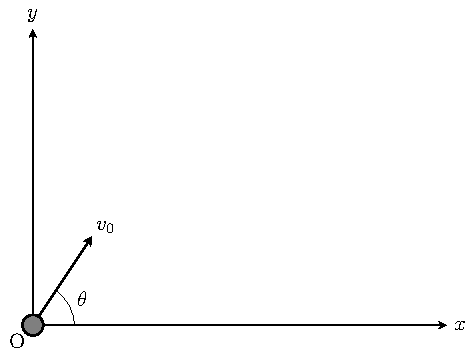
\includegraphics[width=0.75\linewidth]{fig_me_ec_01/fig_me_ec_01_01_a.pdf}
\end{center}

\end{document}
